\cfoot{Samuel Schober}
Im Umfang des Corporate Designs wurden das Logo-Design und das Dokumentdesign behandelt.

\subsubsection{Logo-Design}
Nach teaminterner Besprechung wurde entschieden, dass das Logo in der Farbgebung und dem Design die Grundprinzipien von Aquaponik/Hydroponik darstellen soll. Somit kam der Entschluss, die Farbgebung des Logos, in grün und blau zu setzen (grün stellt die Hydrokultur dar und blau die Aquakultur). Es wurde beschlossen, dass das Design die Initialen des Projektgruppennamen (Urban Green) in minimalistischer Weise umsetzten soll.\\

\begin{figure}[ht]
    \centering
    
\includegraphics[width=0.5\textwidth]{images/ug_Logoproto_1}
	\caption{Urban Green Logoprototyp 1}
\end{figure}

\begin{figure}[ht]
    \centering
	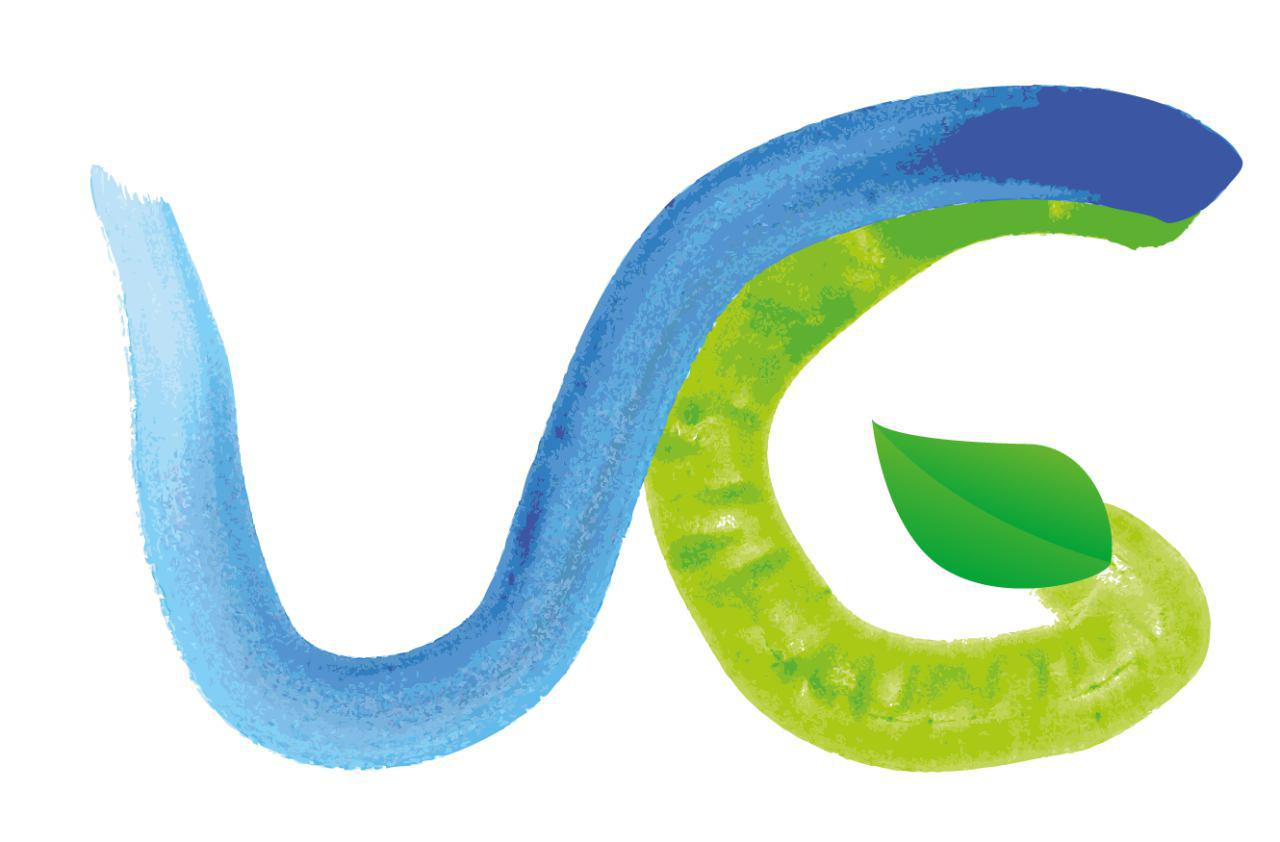
\includegraphics[width=0.5\textwidth]{images/ug_Logoproto_2}
	\caption{Urban Green Logoprototyp 2}
\end{figure}

Alle Logoprototypen waren vom Grundprinzip gleich. Aber die Wahl der Zeichenart entsprach bei den Prototypen nicht den Ansprüchen des Teams. Weitere Gründe, warum diese Prototypen nicht gewählt wurden waren, dass sie den Teammitgliedern ästhetisch nicht gefielen.\\

\begin{figure}[ht]
    \centering
    
\includegraphics[width=0.5\textwidth]{images/ug_Logoproto_3}
	\caption{Urban Green Logoprototyp 3}
\end{figure}
\begin{figure}[ht]
    \centering
	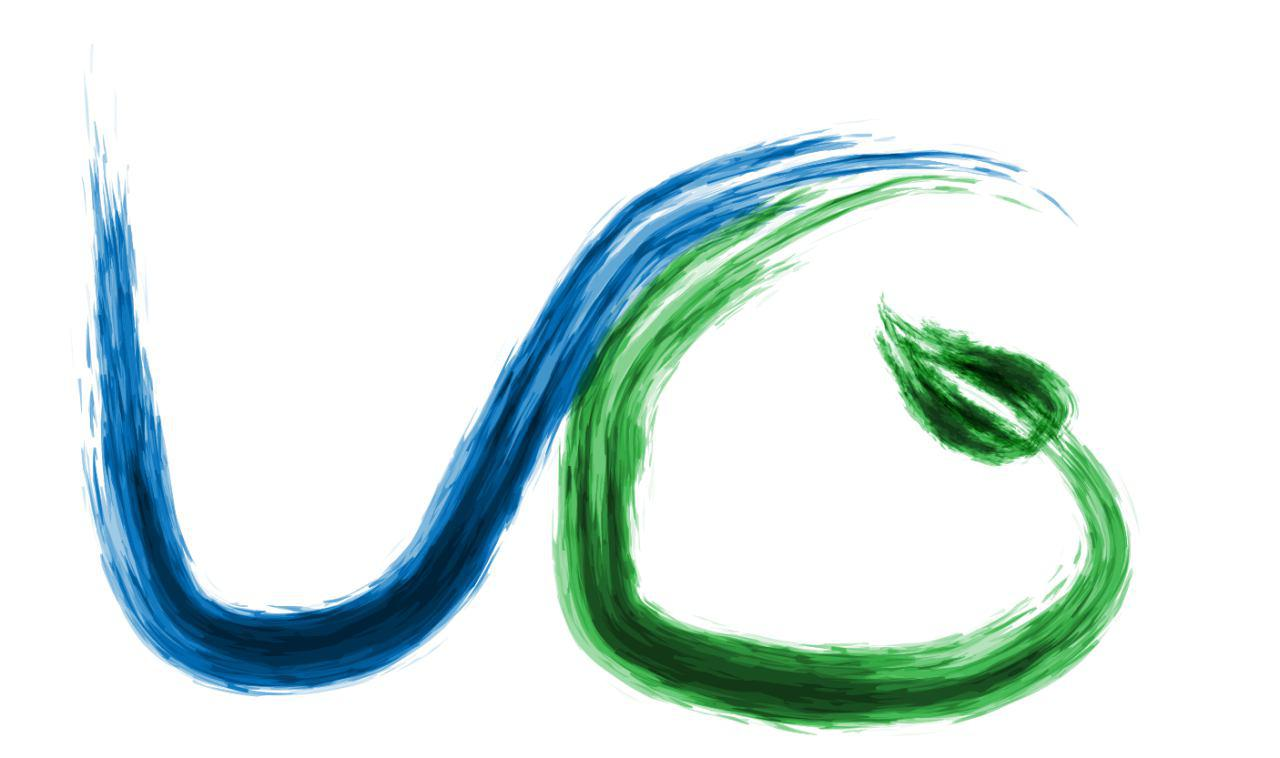
\includegraphics[width=0.5\textwidth]{images/ug_Logoproto_4}
	\caption{Urban Green Logoprototyp 4}
\end{figure}

Durch das Verwenden des Smoke - Illustrator Brush Pack \cite{SmokeBrushSet} (erstellt und gratis zur Verfügung gestellt von DeviantArt Nutzer r2010), konnte ein Schriftzug erstellt werden, der allen Teammitgliedern zusagte. Das Abändern des Blattes in der Mitte des G's und das Anpassen der Form der beiden Buchstaben verhalf, die finale Version des Designs zu erlangen.
\newpage

\begin{figure}[ht]
    \centering
    
\includegraphics[width=0.5\textwidth]{images/logo}
	\caption{Urban Green Logo}
\end{figure}

Hier ist das finale Design des Logos zusehen. Es stellt in einem Schriftzug die beiden Buchstaben U (steht für „Urban“) und G (steht für „Green“) dar. Die Farbgebung ist so gewählt, dass „Green“ grün bleibt und die Hydrokultur darstellt und „Urban“ die Aquakultur darstellt. Als Designeigenschaft wurde bei dem G in der Mitte ein Blatt eingefügt. Das Logo soll den Übergang von Wasser auf den Pflanzensamen darstellen, aus welchem dann die Pflanze wächst.

\subsubsection{Namensgebung der Projektgruppe}
Die Namensgebung unserer Unternehmung sollte ebenso wie das Logo, die Aspekte der Aquaponik/Hydroponik darstellen.\\
Der anfängliche Name „Homeponics“ wurde somit in der Diplomarbeitsdatenbank eingetragen und beschreibt das Homeponics-System, welches im Umfang des Diplomprojekts erstellt wurde. Im Laufe der Abwicklung standen mehrere Namen für das Team zur Auswahl. Schlussendlich wurde „Urban Green“ als Name für das Team gewählt. Das Diplomprojekt behält somit noch immer den Namen „Homeponics“, das Team wird jedoch mit „Urban Green“ bezeichnet.
\newpage

\subsubsection{Dokumentdesign}
Das Dokumentendesign wurde so erstellt, dass die beiden Hauptfarben, grün und blau, als Designelemente eingebaut werden. Als Unterstrichfarbe wurde blau gewählt. Die Designvorlage galt für alle, im Laufe der Projektabwicklungsphase, erstellten Dokumente und Aufzeichnungen. Die Diplomarbeit wurde bewusst ohne diese Designelemente gestaltet, um Normkonformität beizubehalten.\mbox{}\\
\begin{figure}[ht]
    \centering
    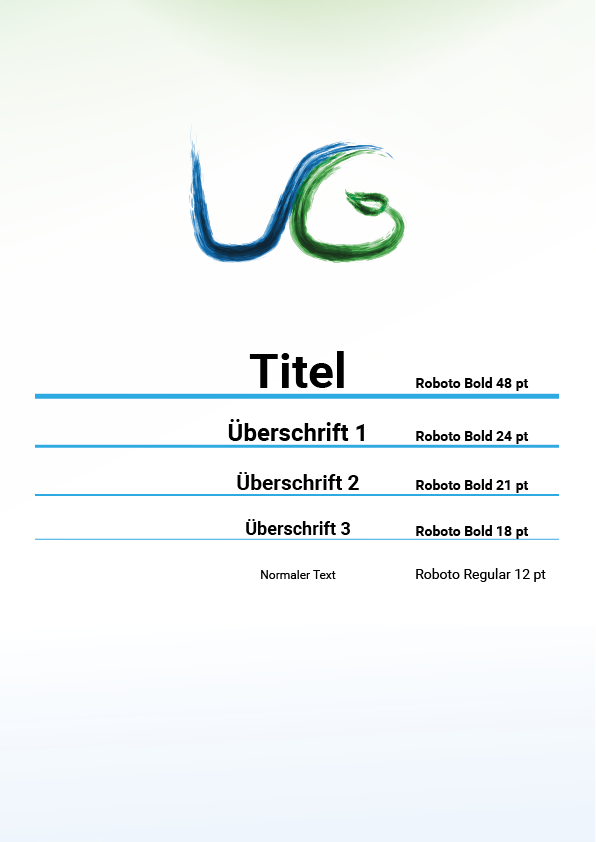
\includegraphics[width=0.7\textwidth]{images/Dokumentdesign}
	\caption{Dokumentdesing-Vorlage}
\end{figure}\textbf{}